%%
%% Figures for additional distance metric.
%% 

\begin{figure*}
  \centering
  \begin{tabular}{ccc}
    
    \begin{minipage}{2in}
      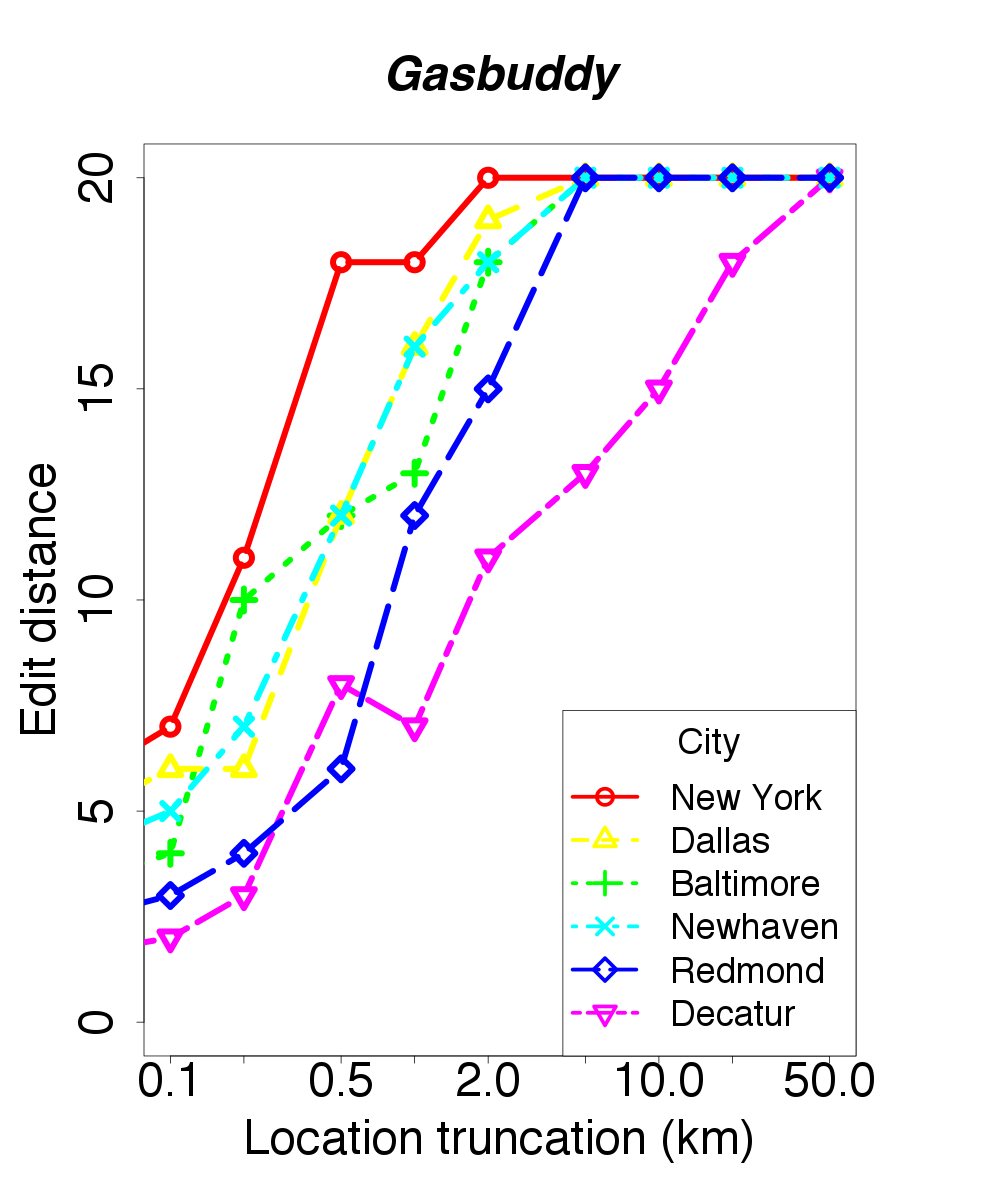
\includegraphics[width=\textwidth]
                      {data/gasbuddy/plots/medians_across_city_20}
    \end{minipage}
    
    % [width=.6\textwidth]
    \begin{minipage}{2in}
      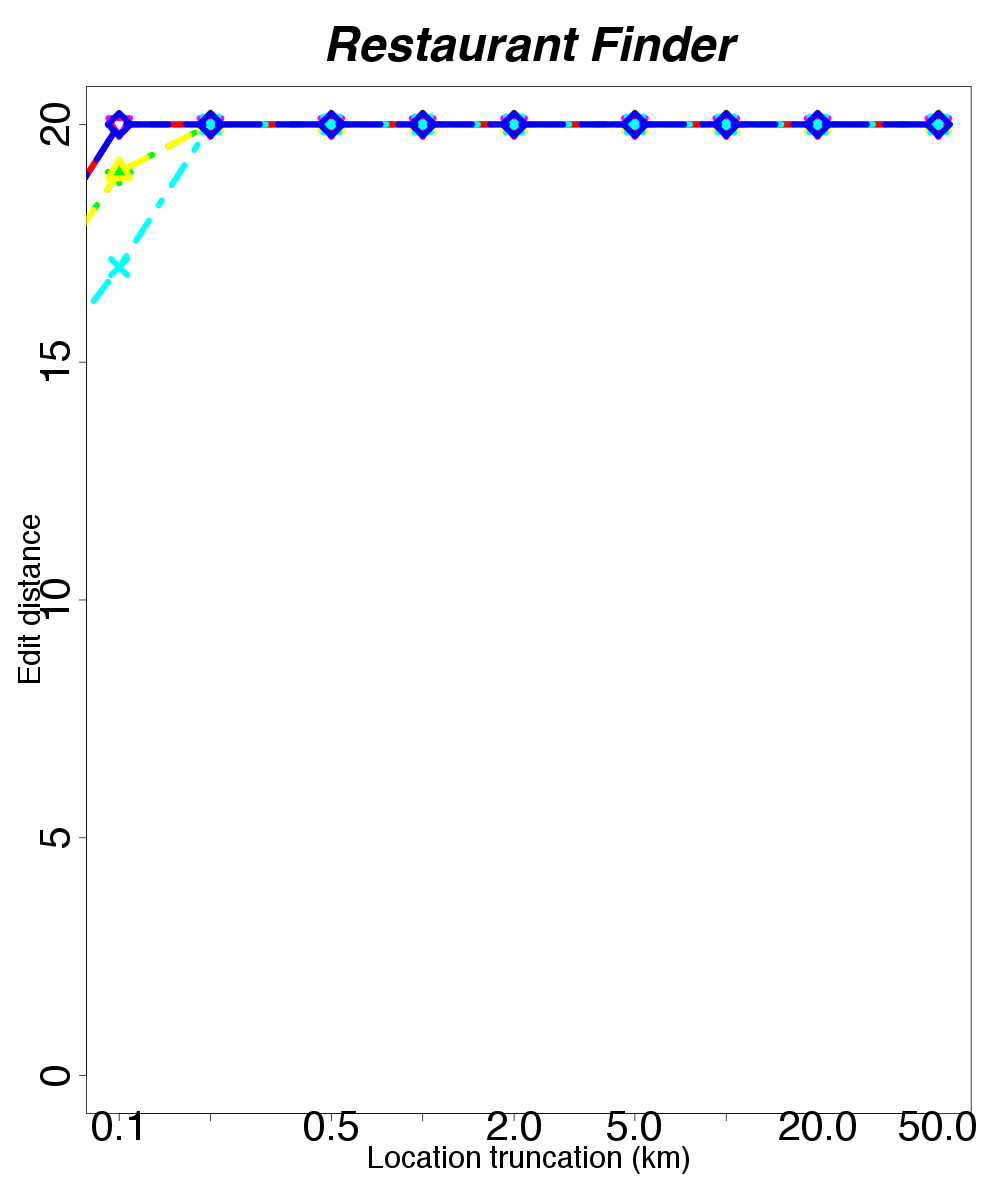
\includegraphics[width=\textwidth]
                      {data/restaurant_finder/plots/medians_across_city_20}
    \end{minipage}
    
    \begin{minipage}{2in}
      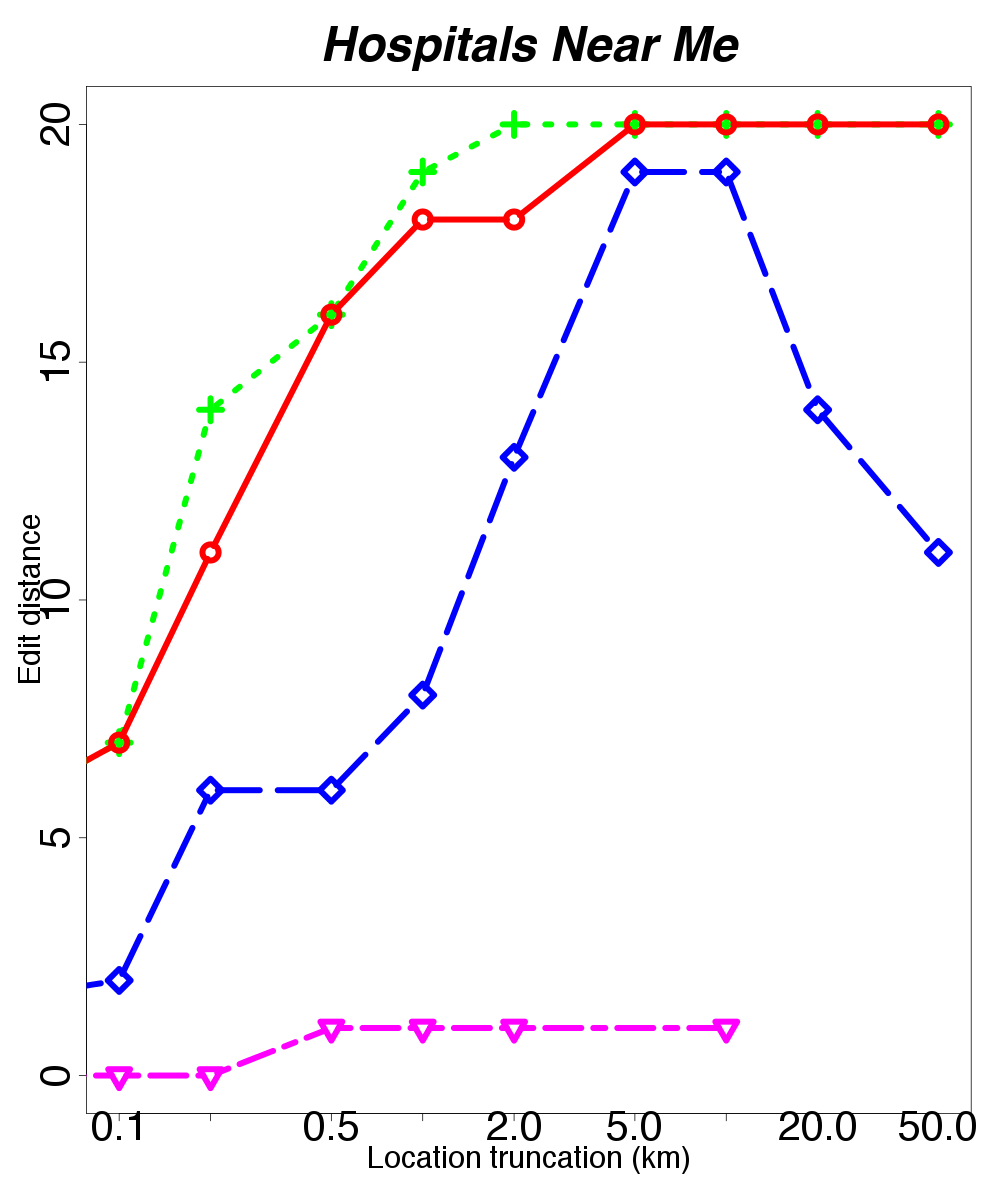
\includegraphics[width=\textwidth]
                      {data/hospitals/plots/medians_across_city_20}
    \end{minipage}
    
    \\
    \begin{minipage}{2in}
      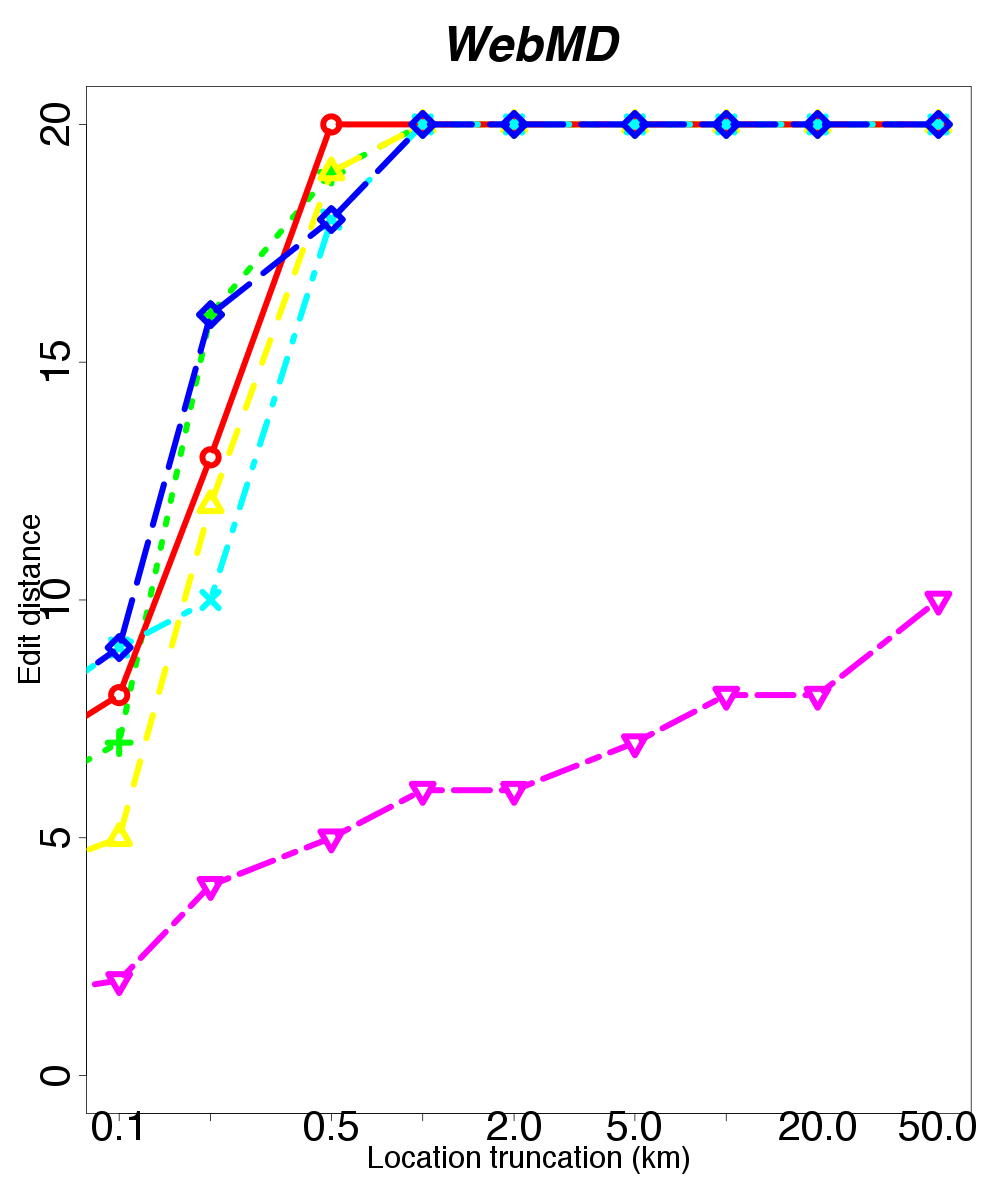
\includegraphics[width=\textwidth]
                      {data/webmd/plots/medians_across_city_20}
    \end{minipage}
    
    \begin{minipage}{2in}
      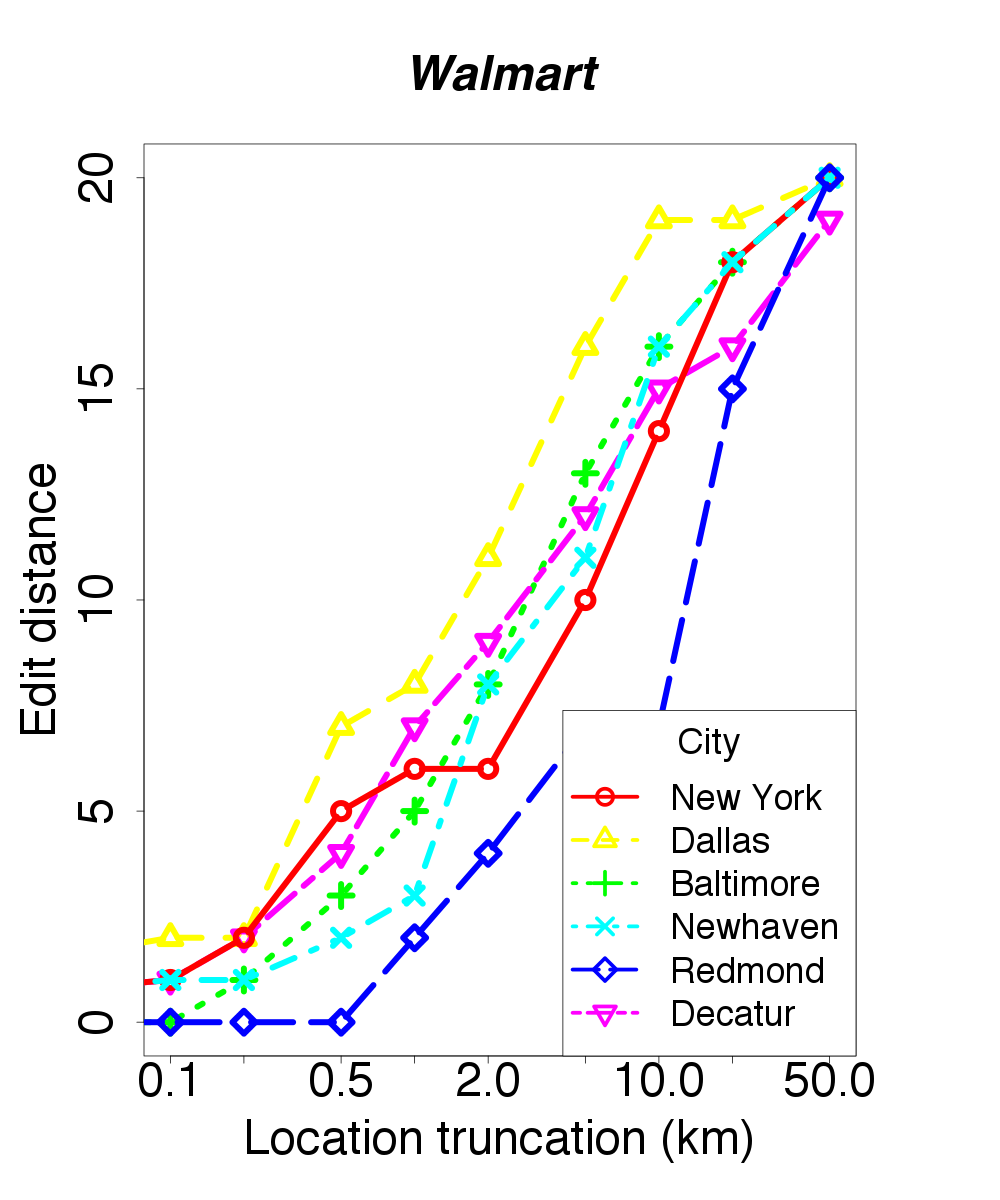
\includegraphics[width=\textwidth]
                      {data/walmart/plots/medians_across_city_20}
    \end{minipage}
    
    \begin{minipage}{2in}
      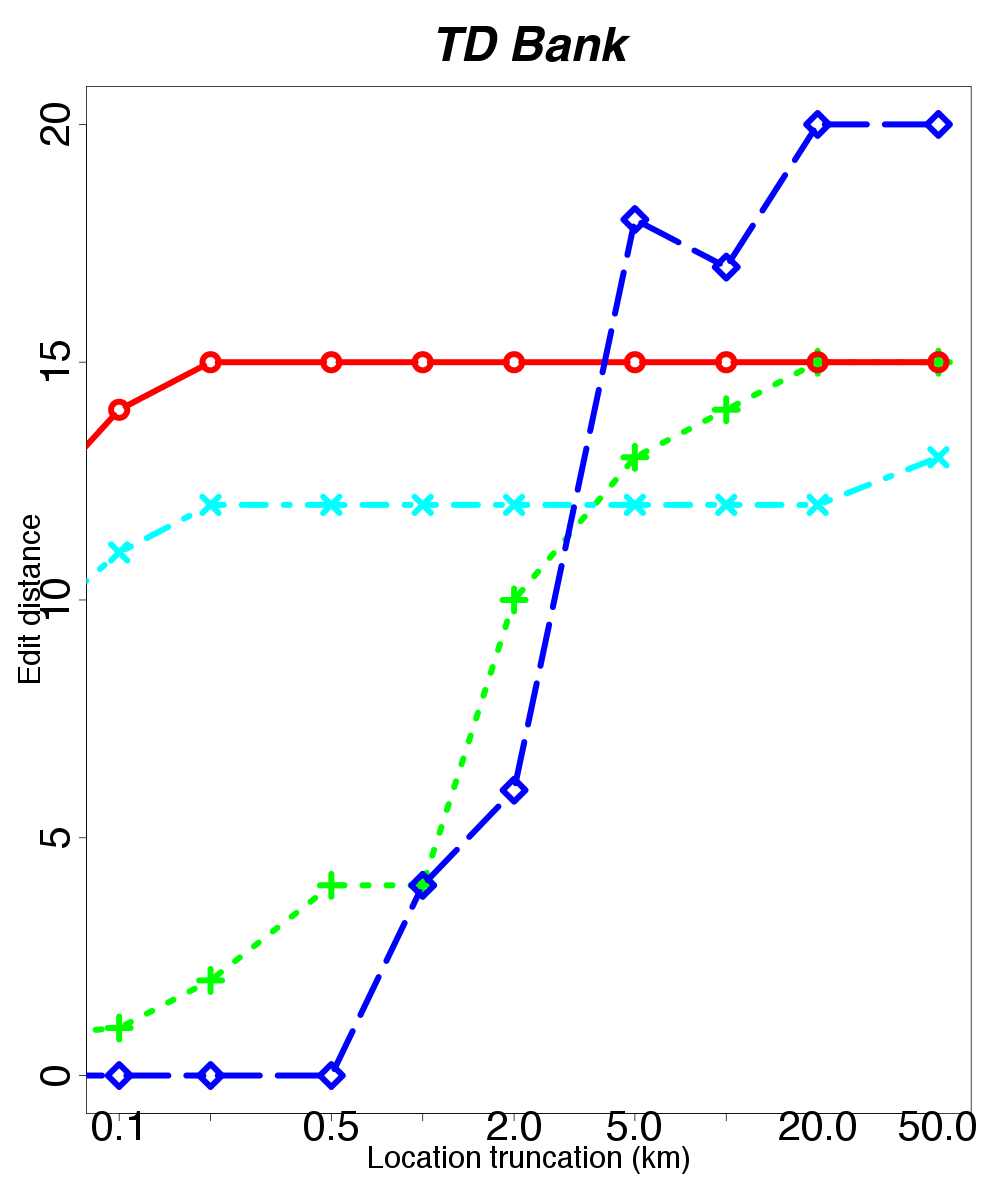
\includegraphics[width=\textwidth]
                      {data/tdbank/plots/medians_across_city_20}
    \end{minipage}
  \end{tabular}
  \caption{The edit intersection metric applied to different apps.  The
    vertical axis indicates the edit distance of the nominal list from 
    the reference list.}
  \label{fig:edit-distance-metric}
\end{figure*}
